\chapter{Introduction}\label{cpt:intro}

Large language models for code generation have moved from laboratory demonstrations to everyday software engineering workflows~\cite{chen2021codex,roziere2023codellama}. Models trained or aligned for programming tasks can produce functions, scripts, tests, data-processing pipelines, and repository patches from natural-language prompts. Their outputs are not static text artifacts: they are compiled, executed, reformatted, translated between languages, edited by humans, and incorporated into larger systems. This property makes provenance and watermarking for generated code both important and technically difficult. A watermark that is visible only in a surface string may disappear after a normal refactoring; a detector that ignores program semantics may flag harmless controls; and a provenance method that damages executable behavior is unlikely to be useful in practice~\cite{kirchenbauer2023watermark,li2023protecting,lee2024who}.

This dissertation is organized around one research question:

\questionbox{How can source-code watermarking be evaluated, embedded, traced, and audited under realistic code-generation conditions?}

The answer developed here is \emph{WatermarkScope}, a benchmark-to-audit framework. I do not treat watermarking as a single binary detector, because the meaning of a detector hit changes with access to the model, the available artifacts, and the risk question being asked. WatermarkScope therefore follows a staged argument. It begins with an executable benchmark for existing runtime watermarking methods, then introduces a structured white-box provenance watermark, and finally moves into black-box null audit, active source attribution, and security triage. In this sequence, \emph{evaluated} maps to CodeMarkBench, \emph{embedded} to SemCodebook, \emph{traced} to CodeDye and ProbeTrace, and \emph{audited} to SealAudit. The ordering matters: fragile benchmark behavior motivates structured provenance; black-box deployment requires a weaker but auditable record; ownership claims require a fixed active-owner registry; and security-sensitive markers require selective review rather than automatic acceptance.

The organizing principle is an \emph{evidence contract}. Each module has to say what kind of observation it produces, which denominator that observation belongs to, and which interpretation it does not support. This is what keeps the dissertation from becoming five unrelated result tables. Formally, a stage is summarized as
\begin{equation}
  \mathcal{L}_j =
  (\mathcal{A}_j,\mathcal{O}_j,\mathcal{D}_j,\mathcal{C}_j,\delta_j,\mathcal{M}_j,\mathcal{I}_j,\mathcal{F}_j),
  \label{eq:lifecycle-stage}
\end{equation}
where $j\in\{\mathrm{benchmark},\mathrm{provenance},\mathrm{audit},\mathrm{attribution},\mathrm{triage}\}$, $\mathcal{A}_j$ is the access model, $\mathcal{O}_j$ is the evidence object, $\mathcal{D}_j$ is the fixed denominator, $\mathcal{C}_j$ is the control set, $\delta_j$ is the frozen decision rule, $\mathcal{M}_j$ is the reported metric vector, $\mathcal{I}_j$ is the allowed interpretation, and $\mathcal{F}_j$ is the set of forbidden interpretations. The lifecycle advances only when $\mathcal{A}_j$ or the risk question changes enough that the previous evidence object cannot support the next claim. This is the main reason CodeDye, ProbeTrace, and SealAudit are not weaker versions of SemCodebook; they answer different evidence questions under different access contracts.

For example, a detector hit in CodeMarkBench is not automatically provenance, contamination evidence, ownership evidence, or safety evidence. It becomes a SemCodebook provenance claim only when the structured carrier and recovery contract is available; it becomes a CodeDye audit signal only when the transcript-bound black-box predicates are frozen; and it becomes a ProbeTrace attribution only under a registered active owner. The same observation therefore changes meaning as the access model changes.

This formalization is stricter than a normal project summary, but the extra discipline is useful. The decision rule $\delta_j$ must be fixed before the result is interpreted; otherwise a later threshold change could turn a diagnostic artifact into an attractive claim. The metric vector $\mathcal{M}_j$ is reported instead of a single portfolio score because recovery, audit yield, attribution, and triage coverage are not the same event. The forbidden set $\mathcal{F}_j$ is also part of the method: a numerical result can look strong and still be scientifically weak if the writing invites a deployment claim that the evidence does not support.

\insightbox{A WatermarkScope result is not just a detector firing. It is a detector output plus an access model, a fixed denominator, a control surface, and a forbidden-claim boundary.}

The five projects are therefore not separate endpoints. Each stage begins where the previous evidence object stops being sufficient: executable benchmarking establishes the denominator, structured carriers support white-box provenance, transcript preservation supports black-box audit, owner registries support scoped attribution, and marker-hidden triage handles security risk. The dissertation's story is the movement from executable evidence to deployable evidence under weaker access and higher governance risk.

\section{Motivation}

Watermarking for ordinary natural language is often evaluated by measuring whether a detector can distinguish generated text from human text under paraphrasing or sampling changes~\cite{kirchenbauer2023watermark,zhao2024provable}. Source code adds several additional constraints. First, generated code has executable semantics: a method that leaves a detectable signal but breaks tests has not solved the practical problem. Second, transformations such as identifier renaming, comment removal, control-flow rewriting, helper extraction, formatting, translation, and dependency repair are normal software operations rather than adversarial edge cases. Third, code-generation systems are often accessed through heterogeneous interfaces: local white-box models, cloud APIs, private fine-tuned students, and benchmark pipelines. Finally, code is security-sensitive. A watermark, marker, or audit prompt may interact with unsafe code patterns, hidden triggers, or provider-level moderation decisions~\cite{pearce2022asleep,perry2023users,siddiq2023llmseceval}.

These constraints motivate a broader evaluation stance. The dissertation asks not only whether a detector fires, but also what denominator it fires on, whether controls remain clean, whether evidence is claim-bearing or support-only, whether uncertainty is reported, and whether the system abstains when evidence is insufficient. This is especially important for avoiding overclaiming. A sparse black-box signal is not a prevalence estimate. A perfect attribution result in one owner setting is not provider-general authorship proof. A selective triage system with high abstention is not an automatic safety classifier.

\section{Design Objectives}

The framework is built around four design objectives. First, results must be executable: a watermark result is not useful if the generated code cannot pass the intended tests. Second, evidence must be denominator-aware: every reported rate must have a fixed claim-bearing denominator and a clear treatment of support-only rows. Third, controls must be explicit: negative controls, false-owner controls, and marker-hidden controls are reported as first-class results rather than buried in implementation notes. Fourth, the system must be allowed to abstain when evidence is insufficient. These objectives are closer to an engineering audit discipline than to a single classifier benchmark.

\section{Lifecycle Framing}

Table~\ref{tab:intro-lifecycle} summarizes how the five stages connect. The important point is that the access model changes across the lifecycle. A white-box provenance method can make stronger claims than a black-box audit, but only within admitted model cells. An active-owner attribution protocol can make stronger source claims than a passive detector, but only after the owner registry is fixed. A safety triage protocol can be useful even with high abstention if it avoids unsafe pass-through. This is why the dissertation reports several evidence surfaces instead of reducing the work to one score.

\begin{table}[htbp]
\centering
\caption{WatermarkScope as one benchmark-to-audit lifecycle.}
\label{tab:intro-lifecycle}
\tighttable
\begin{tabularx}{\textwidth}{@{}L{1.75cm}L{2.15cm}YL{2.35cm}@{}}
\toprule
Stage & Handoff trigger & Evidence object & Claim boundary \\
\midrule
Benchmark & Executability gap & Run inventory and metric vector & Finite release matrix \\
Provenance & Carrier gap & AST/CFG/SSA recovery & Admitted white-box cells \\
Audit & Access gap & Hash-bound transcript evidence & Null audit, not prevalence \\
Attribution & Ownership gap & Owner-bound witness record & Single active owner \\
Triage & Safety gap & Marker-hidden triage row & Selective audit \\
\bottomrule
\end{tabularx}
\end{table}

\section{Contributions}

The dissertation makes five connected contributions. These are contribution points along the same evidence chain, not standalone objectives.

\begin{itemize}
  \item[\stagebullet] \textbf{Benchmark contract}: CodeMarkBench provides an executable benchmark foundation with four pinned runtime baselines, five local code models, seven benchmark source groups, and a canonical 140/140 run-completion matrix. The repository entry points are recorded in Appendix~\ref{app:repository-access}.
  \item[\stagebullet] \textbf{White-box provenance}: SemCodebook uses AST, CFG, and SSA carrier families with keyed scheduling and error-correcting recovery for admitted white-box model cells.
  \item[\stagebullet] \textbf{Black-box audit}: CodeDye preserves hash-bound raw-response and structured evidence while refusing to infer contamination prevalence from sparse signals.
  \item[\stagebullet] \textbf{Source attribution}: ProbeTrace uses owner registries, semantic witnesses, decoys, and false-owner controls for active-owner, source-bound attribution.
  \item[\stagebullet] \textbf{Security triage}: SealAudit reports marker-hidden selective triage, explicit needs-review outcomes, and unsafe-pass boundaries.
\end{itemize}

\begin{figure}[!t]
  \centering
  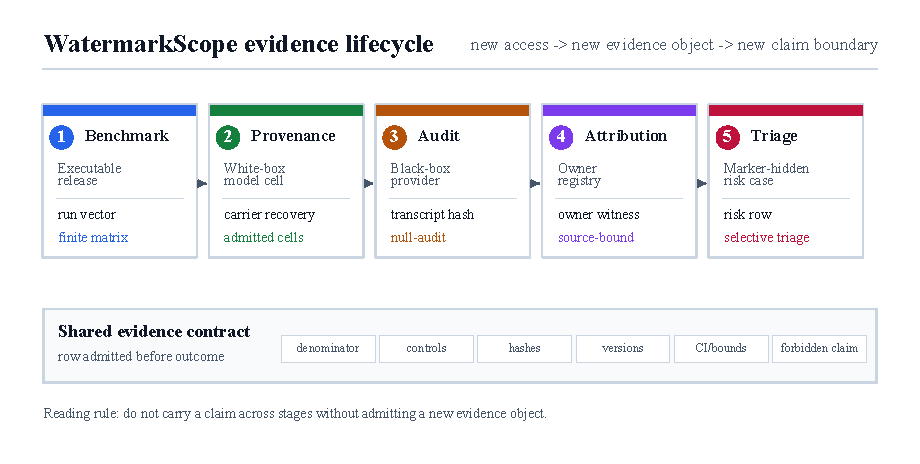
\includegraphics[width=\textwidth]{fig/watermarkscope_framework_map.pdf}
  \caption{WatermarkScope evidence lifecycle. A new access model creates a new evidence object and claim boundary; claims do not transfer across stages without a new admitted surface.}
  \label{fig:watermarkscope-pipeline}
\end{figure}

\section{Threat Model and Evaluation View}

The threat model assumes that generated code may be transformed by normal developer actions or by deliberate laundering attempts. Such transformations include identifier renaming, comment stripping, formatting changes, helper extraction, control-flow rewriting, cross-language translation, and query-budget changes in black-box audits. The defender or auditor may have white-box access to a local model in SemCodebook, black-box transcript access in CodeDye, a registered active-owner key in ProbeTrace, or only marker-hidden audit evidence in SealAudit. The thesis therefore uses different claim types for different access models instead of pretending that one detector can answer all provenance questions.

\section{Scope and Non-Claims}

The dissertation is careful about scope. CodeMarkBench does not prove that all source-code watermarking fails; it evaluates the included runtime baselines under the included models, source groups, and stress conditions. SemCodebook does not claim universal semantic watermarking; it claims structured provenance recovery within admitted white-box family and scale cells. CodeDye does not accuse a model provider of contamination and does not estimate contamination prevalence. ProbeTrace does not claim provider-general or multi-owner attribution. SealAudit does not certify watermark harmlessness or provide an automatic safety classifier. These limits are not apologies for the work. They are the boundaries that make the results checkable.

This scoping also defines how the implementation should be inspected. The submitted WatermarkScope repository is the FYP artifact: it contains the dissertation source, method snapshots, result manifests, preserved evidence summaries, and examiner-facing verification scripts. CodeMarkBench is separately listed because it is an earlier benchmark artifact that supplies the executable foundation for the first stage. It should be read as supporting infrastructure for the lifecycle, not as a second dissertation. Appendix~\ref{app:repository-access} lists both access points and explains which repository should be used for marking.

The distinction matters for assessment. A design project is not complete when a PDF describes an idea; it must expose enough implementation structure for an examiner to inspect how the evidence was generated, which files bind to the printed claims, and which checks can be rerun without private keys or GPUs. For this reason, the report treats code and manifests as part of the argument rather than as optional supplementary material. The writing names the evidence surfaces, but the repository supplies the artifact paths, hashes, and scripts that make those surfaces auditable.

The remaining chapters follow the same lifecycle order: background, executable benchmark foundation, white-box and black-box evidence protocols, attribution and security triage, and finally a synthesis of confidence intervals, claim boundaries, and future work. This order is part of the argument. Each chapter changes the evidence object only when the previous access model can no longer support the next claim, and the report avoids a single portfolio score because recovery, audit yield, attribution, and triage coverage are different events rather than interchangeable measurements.

The reader should therefore track two threads at the same time. The first thread is technical: how to build benchmark rows, structured carriers, transcript-bound audit records, owner witnesses, and marker-hidden triage rows. The second thread is evidential: how each row becomes admissible, which denominator it enters, and which interpretation is deliberately blocked. A strong result in this dissertation is not simply the largest numerator. It is a result whose numerator is tied to a stable denominator, whose controls make the failure modes visible, and whose wording does not move beyond the access model that produced the evidence. The following chapter therefore reviews benchmarks, watermarking, provenance, and security as evidence problems rather than as isolated literatures.

This reading lens is also the standard used to judge the submitted design artifact. A technically strong implementation is not enough if the written claim moves faster than the evidence; a carefully scoped claim is not enough if the repository cannot show how the row was produced. WatermarkScope is intended to satisfy both requirements at once. The chapters therefore alternate between method design and evidence accounting: each protocol is introduced through the access assumption that makes it possible, the records that make it auditable, and the boundary that stops it from becoming a broader claim than the experiment supports.

This also explains the report's treatment of negative results and abstentions. The benchmark chapter does not hide baseline tradeoffs; the white-box chapter keeps misses inside the recovery denominator; the black-box chapter reports sparse signals as sparse; the attribution chapter writes a perfect scoped result as scoped; and the triage chapter treats review load as an outcome rather than a nuisance. These choices make the dissertation less sensational, but they make it more inspectable. A reader should be able to ask, for every number in the report, four questions: what was counted, what was excluded before the outcome was known, what control surface was used, and what conclusion is forbidden. The rest of the dissertation is organized to answer those questions in the same order as the lifecycle.
